% IMPORTANT: PLEASE USE XeLaTeX FOR TYPESETTING
\documentclass[10pt]{beamer}

\usetheme{Darmstadt}%{default}
\usecolortheme{beaver}
\usepackage[T1]{fontenc} 
\usepackage[utf8]{inputenc}
\usepackage[french]{babel}
\usefonttheme{serif}
\usepackage{lmodern}
\usepackage{tcolorbox}
 % pour un pdf lisible à l'écran
 % il y a d'autres choix possibles 
\usepackage{pslatex}
% \usepackage{ctex, hyperref}
\usepackage{latexsym,amsmath,xcolor,multicol,booktabs,calligra}
\usepackage{graphicx,pstricks,listings,stackengine}
\usepackage{chemfig}

\usepackage{tabularx}
% meta-data
\title{Leçon :Effet tunnel, radioactivité $\alpha$}

\author{Gabriel Le Doudic}
\institute{Préparation à l'agrégation de Rennes}
% \titlebackground{images/background}

\definecolor{aquamarine}{rgb}{0.5, 1.0, 0.83}
\definecolor{applegreen}{rgb}{0.55, 0.71, 0.0}	
\definecolor{cobalt}{rgb}{0.0, 0.28, 0.67}

\definecolor{definitionf}{RGB}{220,252,220}
\definecolor{definitionl}{RGB}{39,123,69}
\definecolor{definitiono}{RGB}{72,148,101}

\definecolor{propositionf}{RGB}{255,216,218}
\definecolor{propositionl}{RGB}{38,38,38}
\definecolor{propositiono}{RGB}{109,109,109}

\definecolor{theof}{RGB}{255,216,218}
\definecolor{theol}{RGB}{160,0,4}
\definecolor{theoo}{RGB}{221,65,100}

\definecolor{avertl}{RGB}{163,92,0}
\definecolor{averto}{RGB}{255,144,0}

\definecolor{histf}{RGB}{241,238,193}

\definecolor{metf}{RGB}{220,230,240}
\definecolor{metl}{RGB}{56,110,165}
\definecolor{meto}{RGB}{109,109,109}


\definecolor{remf}{RGB}{230,240,250}
\definecolor{remo}{RGB}{150,150,150}

\definecolor{exef}{RGB}{240,240,240}

\definecolor{protf}{RGB}{247,228,255}
\definecolor{protl}{RGB}{105,0,203}
\definecolor{proto}{RGB}{174,88,255}

\definecolor{grid}{RGB}{180,180,180}

\definecolor{titref}{RGB}{230,230,230}

\definecolor{vert}{RGB}{23,200,23}

\definecolor{violet}{RGB}{180,0,200}

\definecolor{copper}{RGB}{217, 144, 88}
%% CADRES

\newtcolorbox{defi}[1]{
	colback=applegreen!5!white,
  	colframe=applegreen!65!black,
	fonttitle=\bfseries,
  	title={#1}}
\newtcolorbox{Programme}[1]{
	colback=cobalt!5!white,
  	colframe=cobalt!65!black,
	fonttitle=\bfseries,
  	title={#1}}  
\newtcolorbox{Resultat}[1]{
	colback=theof,%!5!white,
	colframe=theoo!85!black,
  fonttitle=\bfseries,
	title={#1}} 
\usepackage{tikz}
\usepackage{array}
\usepackage[scientific-notation=true]{siunitx}
\usetikzlibrary{matrix}
\newcommand{\diff}{\mathrm{d}}

\title{Leçon : Transition de phase}

% document body
\begin{document}
\begin{frame}{}
    \titlepage

    \begin{tabularx}{\textwidth}{l@{:\,\,}X}
        \textbf{Niveau} 	  & CPGE\\
        \textbf{Prérequis} & notion de système et d'equilibre thermodynamique \\
        & transformations classiques en thermodynamique \\
        & premier et second principe
    \end{tabularx}
\end{frame}

\begin{frame}
    \tableofcontents
\end{frame}

\section{États de la matière}
\subsection{Trois phases principales}

\begin{frame}{\insertsubsection}
    \begin{figure}
        \centering
        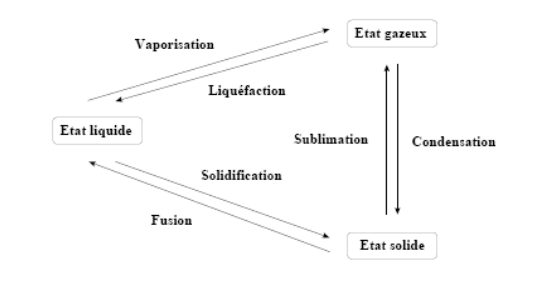
\includegraphics[width= .8\textwidth]{EtatMatiere.png}
        \caption{Cours thermo Paris Saclay Bobroff, Puzo}
    \end{figure}
\end{frame}

\begin{frame}{\insertsubsection}
    \begin{figure}
        \centering
        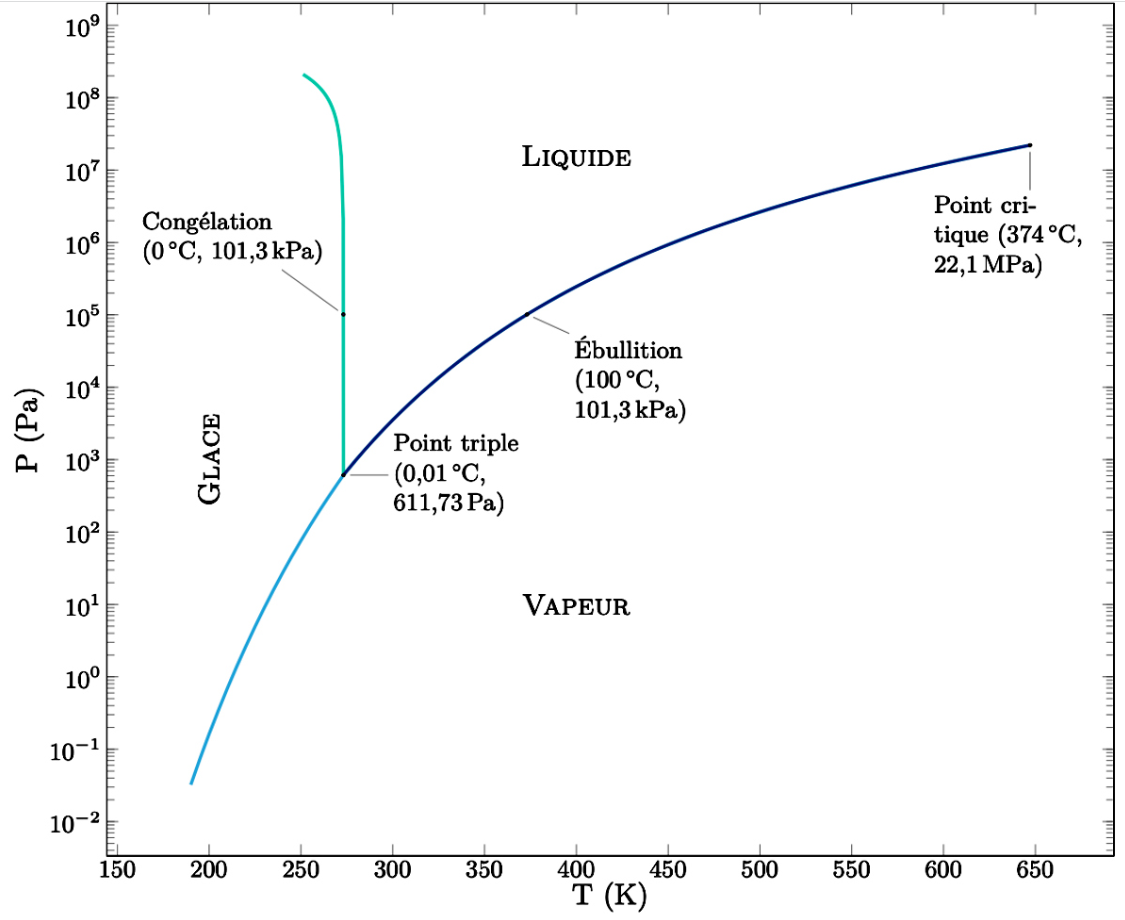
\includegraphics[width= .7\textwidth]{Point_triple_deleau_enslyon.png}
        \caption{\href{https://planet-terre.ens-lyon.fr/ressource/diagramme-lineaire-log.xml}{eduscol ens de lyon}}
    \end{figure}
\end{frame}

\subsection{Corps purs}

\section{Transitions solide-liquide vapeur}
\subsection{Diagrammes des variables d'état}

\begin{frame}{\insertsubsection}
    \begin{minipage}{.48\linewidth}
    \begin{figure}
        \centering
        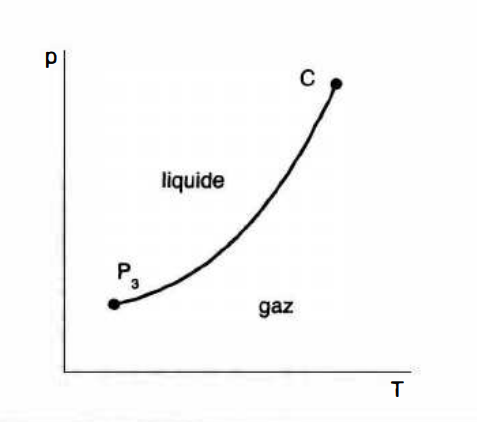
\includegraphics[width=1\textwidth]{Courbe_vaporisation_Diu.png}
        \caption{Courbe de vaporisation Diu p300}
    \end{figure}
    \end{minipage}
    \begin{minipage}{.48\linewidth}
    \begin{figure}
        \centering
        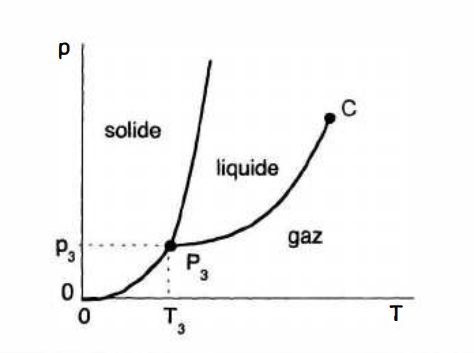
\includegraphics[width=1.1\textwidth]{Diagramme_corps_purs.png}
        \caption{Courbe de vaporisation Diu p301}
    \end{figure}
\end{minipage}
\end{frame}


\begin{frame}{\insertsubsection}
    % \begin{minipage}{.48\linewidth}
    \begin{figure}
        \centering
        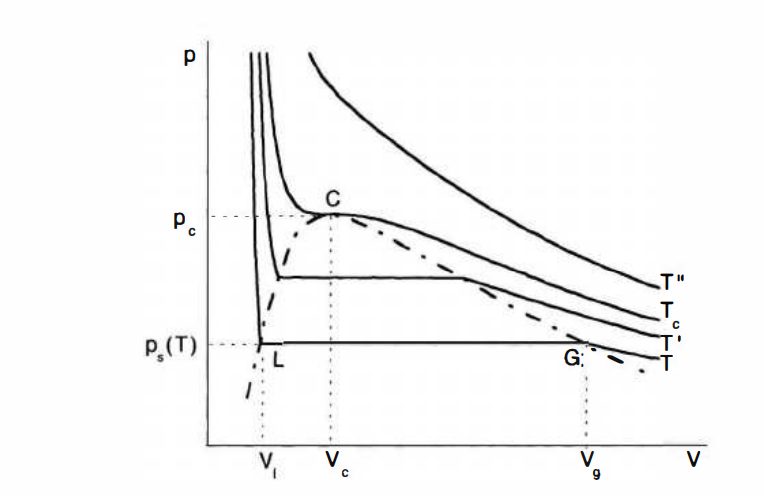
\includegraphics[width=.8\textwidth]{Isotherme_courbe_vaporisation.png}
        \caption{Courbe de vaporisation Diu p300}
    \end{figure}
    \href{https://www.youtube.com/watch?v=nxAdQ_8tC1U&ab_channel=Unisciel}{Bouillant de Franklin}
% \end{minipage}
% \begin{minipage}{.48\linewidth}
%     \begin{figure}
%         \centering
%         %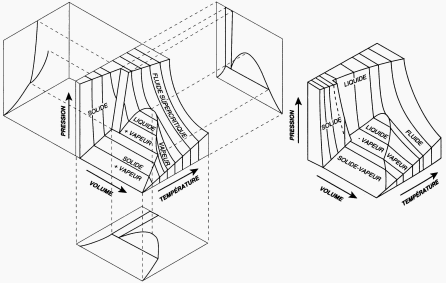
\includegraphics[width=1\textwidth]{DiagrammePVT.png}

%         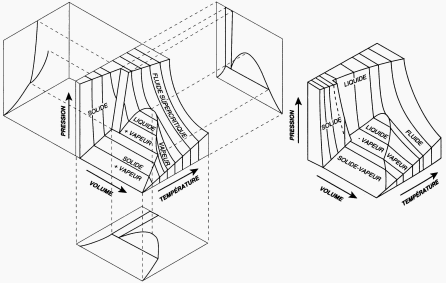
\includegraphics[width=1.2\textwidth]{DiagrammePVT.png}
%         \caption{Diagramme P,V et T pour un corps pur}
%     \end{figure}
% \end{minipage}
\end{frame}

\begin{frame}{\insertsubsection}
    \begin{figure}
        \centering
        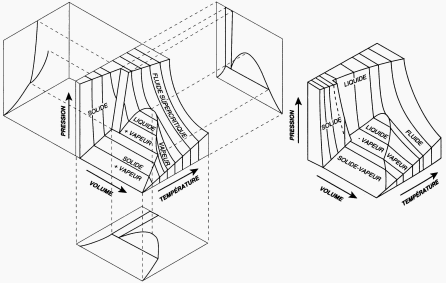
\includegraphics[width=1\textwidth]{DiagrammePVT.png}
        \caption{Diagramme P,V,T}
    \end{figure}
\end{frame}



\subsection{Étude thermodynamique d'une transition de phase du premier ordre}
\subsection{Mesure de la chaleur latente de vaporisation du diazote}
\subsection{Retard à la transition de phase: metastabilité}
\section{Transitions ferro para, transition du second ordre}
\subsection{Modèle}
\begin{frame}{\insertsubsection}
    \textbf{Modèle de Landau (expression générale):}
    \begin{equation}
        G(T,M) = A_0(T)+\alpha(T)M^2+\frac{1}{2}\beta(T)M^4+...
    \end{equation}

    \textbf{Minimisation du potentiel (deux coniditions):}
    \begin{equation}
        \begin{array}{cc}
            \left. \dfrac{\partial G}{\partial M}\right|_T = 0, &\left. \dfrac{\partial^2G}{\partial M^2}\right|_T >0\\
            2\alpha M+2\beta M^3 = 0, & 2\alpha + 6\beta M^2 >0.
        \end{array}
    \end{equation}
    \textbf{Solutions possibles:} 
    \begin{equation}
        \begin{array}{cc}
            M_1=0,  & M_2=\left(-\dfrac{\alpha}{\beta}\right)^{1/2}\\
            \left. \dfrac{\partial^2 G}{\partial M^2}\right|_T (M_1)=2\alpha, & \left.\dfrac{\partial^2 G}{\partial M^2}\right|_T(M_2)=-4\alpha.
        \end{array}
    \end{equation}

\end{frame}
\subsection{Comparaison aux résultats expérimentaux}
\begin{frame}{\insertsubsection}
    \begin{itemize}
        \item Quand $T<T_c$, $M>0$, ce qui impose $\alpha$ et $\beta$ de signes opposés. On veut aussi une solution stable:
        \begin{equation}
            \left.\dfrac{\partial^2G}{\partial M^2}\right|_T(M=\sqrt{-\alpha/\beta})= 2\alpha+6\beta M^2=-4\alpha>0.
        \end{equation}
        Donc $\alpha<0$
        \item Quand $T=T_c$, $M_2$ tend vers 0, en ce point on veut une stabilité donc :
        \begin{equation}
            \left. \dfrac{\partial^2G}{\partial M^2}\right|_T\approx 2\alpha+6\beta M^2>0 \rightarrow \beta>0.
        \end{equation}
        \item Quand $T>T_c$, On veut $M=0$ et une solution stable. Cette fois cela impose :
        \begin{equation}
            \left. \dfrac{\partial^2G}{\partial M^2}\right|_T(M=0)=2\alpha>0.
        \end{equation}
        par continuité avec $T_c$, $\beta$ est positif aussi.
    \end{itemize}
\end{frame}

\begin{frame}{\insertsubsection}
    \begin{itemize}
        \item $\beta = \beta_c>0$ car ne change pas de signe 
        \item $\alpha(T) = a(T-T_c)$ avec $a>0$.
    \end{itemize}
    \begin{equation}
        G(T,M)\approx A_0(T) + a(T-T_c)M^2+\dfrac{\beta_c}{2}M^4
    \end{equation}
    \begin{minipage}{.48\linewidth}
    \begin{figure}
        \centering
        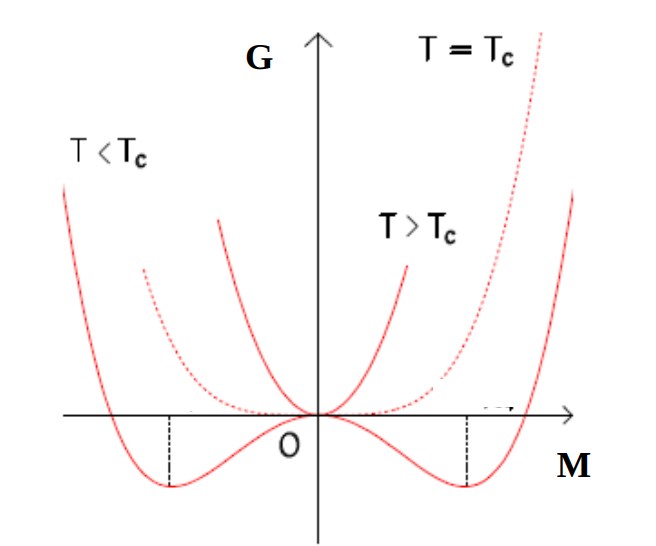
\includegraphics[width=1\textwidth]{Ferro_para.png}
    \end{figure}
\end{minipage}
\begin{minipage}{.48\linewidth}
    Le Modèle prédit au voisinage de $T_c$:
    \begin{equation}
        M(T<T_c) = \sqrt{\dfrac{a}{\beta}(T_c-T)} 
    \end{equation}

\end{minipage}
\end{frame}
\end{document}